\section{Fundamentals of architecture}

The main purpose of this chapter is to introduce some basics of parallel computing theory. It will introduce the simplest and trivial processor and the more complex and efficient variants. The topics introduced are explained in a simple way and without any deepening, because it is only an introduction. For those who have studied computer science, this chapter might be a little boring and you might notice that some topics are explained in a simplistic way.

\longline

\subsection{Introduction}

\subsubsection{Simplest processor}

Inside a computer, a processor executes instructions.
\begin{itemize}
    \item \textbf{Fetch/Decode}: Determine which instruction to run next;
    \item \textbf{ALU} (execution unit): Performs the operation described by an instruction, which may change values in the processor's registers or the computer's memory;
    \item \textbf{Registers}: maintain program state, store values of variables used as inputs and outputs to operations.
\end{itemize}
The simplest and most basic processor executes \textbf{one instruction per clock cycle}.
\begin{figure}[!htp]
    \centering
    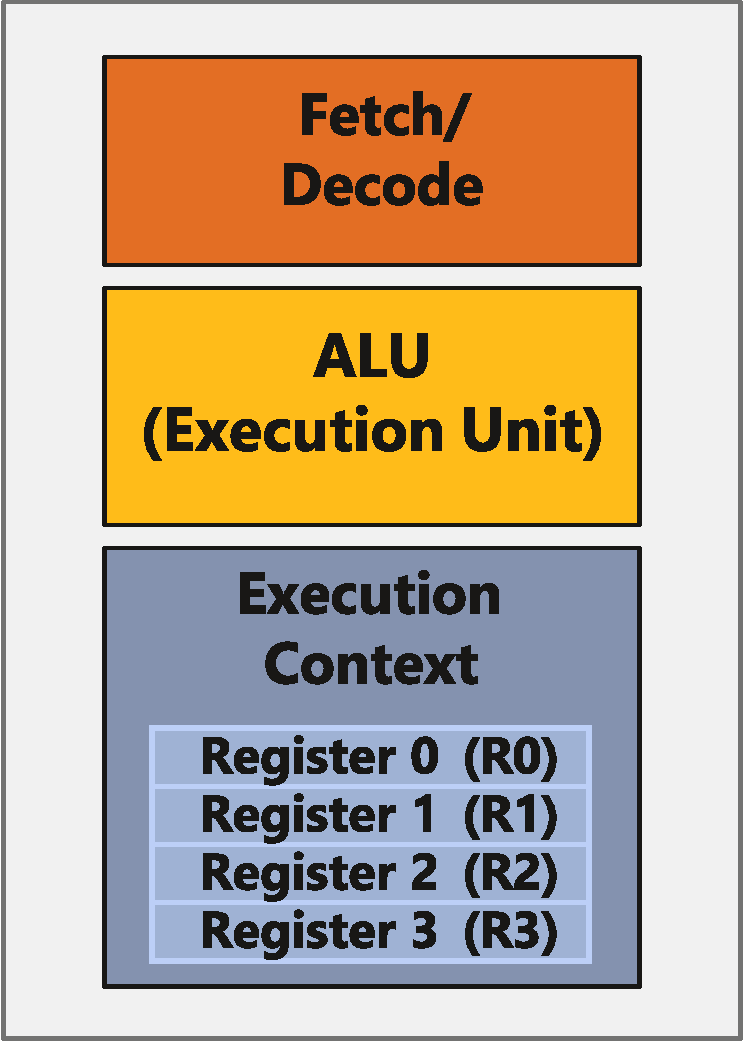
\includegraphics[width=.3\textwidth]{img/simplest-prcoessor-1.pdf}
    \caption{The simplest and most basic processor.}
\end{figure}

\newpage

\subsubsection{Superscalar processor}
A more \dquotes{complex} and realistic model is the \definitionWithSpecificIndex{superscalar processor}{Superscalar Processor}{}. This \textbf{processor can decode and execute up to \underline{two instructions per clock}}. The execution is slightly different from the simplest processor. The \textbf{processor automatically finds independent instructions in an instruction sequence and can execute them in parallel on multiple execution units}.
\begin{figure}[!htp]
    \centering
    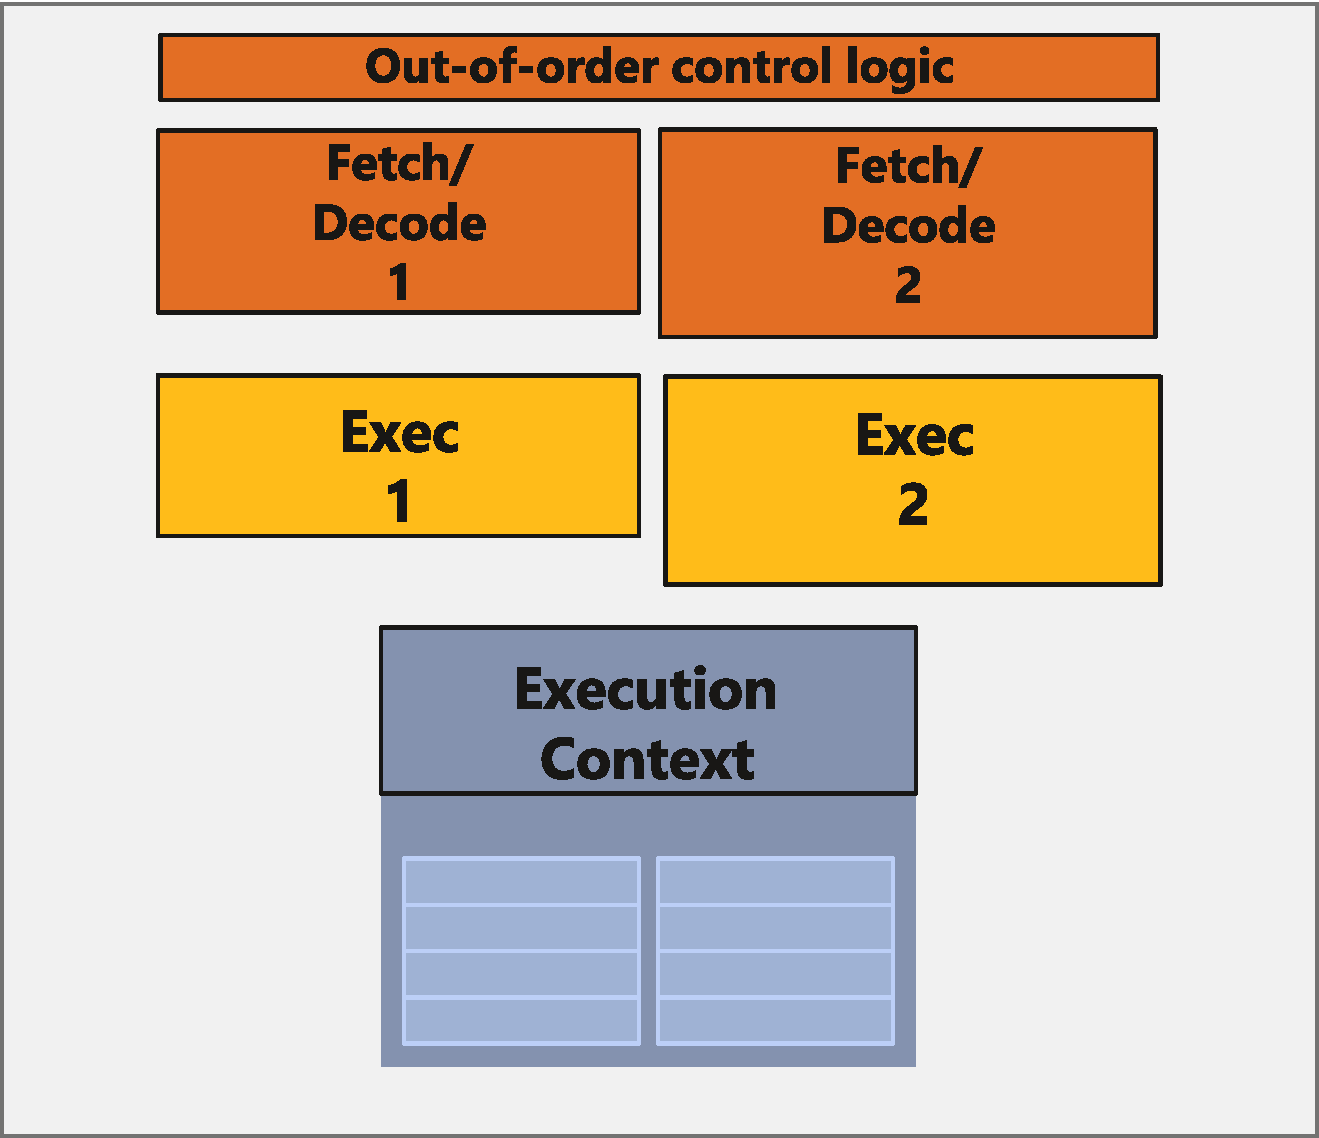
\includegraphics[width=.52\textwidth]{img/superscalar-prcoessor-1.pdf}
    \caption{The superscalar processor.}
\end{figure}

\noindent
The superscalar processor takes advantage of \definition{Instruction-Level Parallelism (ILP)}\footnote{Instruction-level parallelism (ILP) is the parallel or simultaneous execution of a sequence of instructions in a computer program. More specifically ILP refers to the average number of instructions run per step of this parallel execution.} within an instruction stream.
\begin{itemize}
    \item Processing \textbf{different instructions} from the same instruction stream \textbf{in parallel} (\textbf{within a core}).
    \item \textbf{Parallelism is automatically detected by the hardware during execution}.
\end{itemize}

\newpage

\subsubsection{Single Instruction, Multiple Data (SIMD) processor}\label{subsubsection: Single Instruction, Multiple Data (SIMD) processor}

Adding execution units (ALUs) to the simplest processor can increase compute capability. Amortize the cost/complexity of managing an instruction stream across many ALUs using \definition{Single Instruction, Multiple Data (SIMD)} processing. Therefore, the \textbf{same instruction is sent to all ALUs}. This \textbf{operation is performed in parallel on all ALUs}.

\begin{flushleft}
    \textcolor{Green3}{\faIcon{check} \textbf{Advantages}}
\end{flushleft}
\begin{itemize}
    \item \textbf{Efficient for data-parallel workloads}: amortize control costs over many ALUs.
    \item Vectorization done by:
    \begin{itemize}
        \item Compiler (\textbf{\underline{explicit SIMD}}): parallelism is explicitly requested by the programmer through intrinsics, conveyed through parallel language semantics, and inferred through loop dependency analysis by the \dquotes{auto-vectorizing} compiler. In other words, the \textbf{SIMD parallelization is done at compile time, and when we inspect the program binary, we can see the SIMD instructions}.

        \item At runtime by hardware (\textbf{\underline{implicit SIMD}}): the \textbf{compiler generates a binary with scalar instructions}, but $n$ instances of the program are always executed together on the processor. The \textbf{hardware} (not the compiler) is \textbf{responsible for the simultaneous execution of the same instruction by multiple program instances on different data on SIMD ALUs}.
    \end{itemize}
\end{itemize}

\longline

\subsubsection{Multi-Core Processor}

A \definition{Multi-Core Processor (MCP)} is a \textbf{microprocessor} on a single integrated circuit (IC) with \textbf{two or more separate central processing units (CPUs)}, called \emph{cores} to emphasize their multiplicity (e.g., \emph{dual-core} or \emph{quad-core}). Each core reads and executes program instructions, specifically ordinary CPU instructions (such as \texttt{add}, \texttt{move data}, and \texttt{branch}). However, the MCP can \textbf{execute instructions on separate cores simultaneously}, \textbf{increasing overall speed for programs that support multithreading or other parallel computing techniques}.
\begin{flushleft}
    \textcolor{Green3}{\faIcon{check} \textbf{Advantages}}
\end{flushleft}
\begin{itemize}
    \item Provides \textbf{thread-level parallelism}: execute a completely different instruction stream on each core simultaneously.
    \item \textbf{Software creates threads to expose parallelism to hardware} (e.g., via threading API)
\end{itemize}